% =============================================================================
% Nova Fun & Games - Cover Page
% =============================================================================
\IfFileExists{assets/front-cover.png}{%
\begin{titlepage}
\thispagestyle{empty}
\begin{tikzpicture}[remember picture, overlay]
  \fill[black] (current page.south west) rectangle (current page.north east);
  \node[inner sep=0pt] at (current page.center)
    {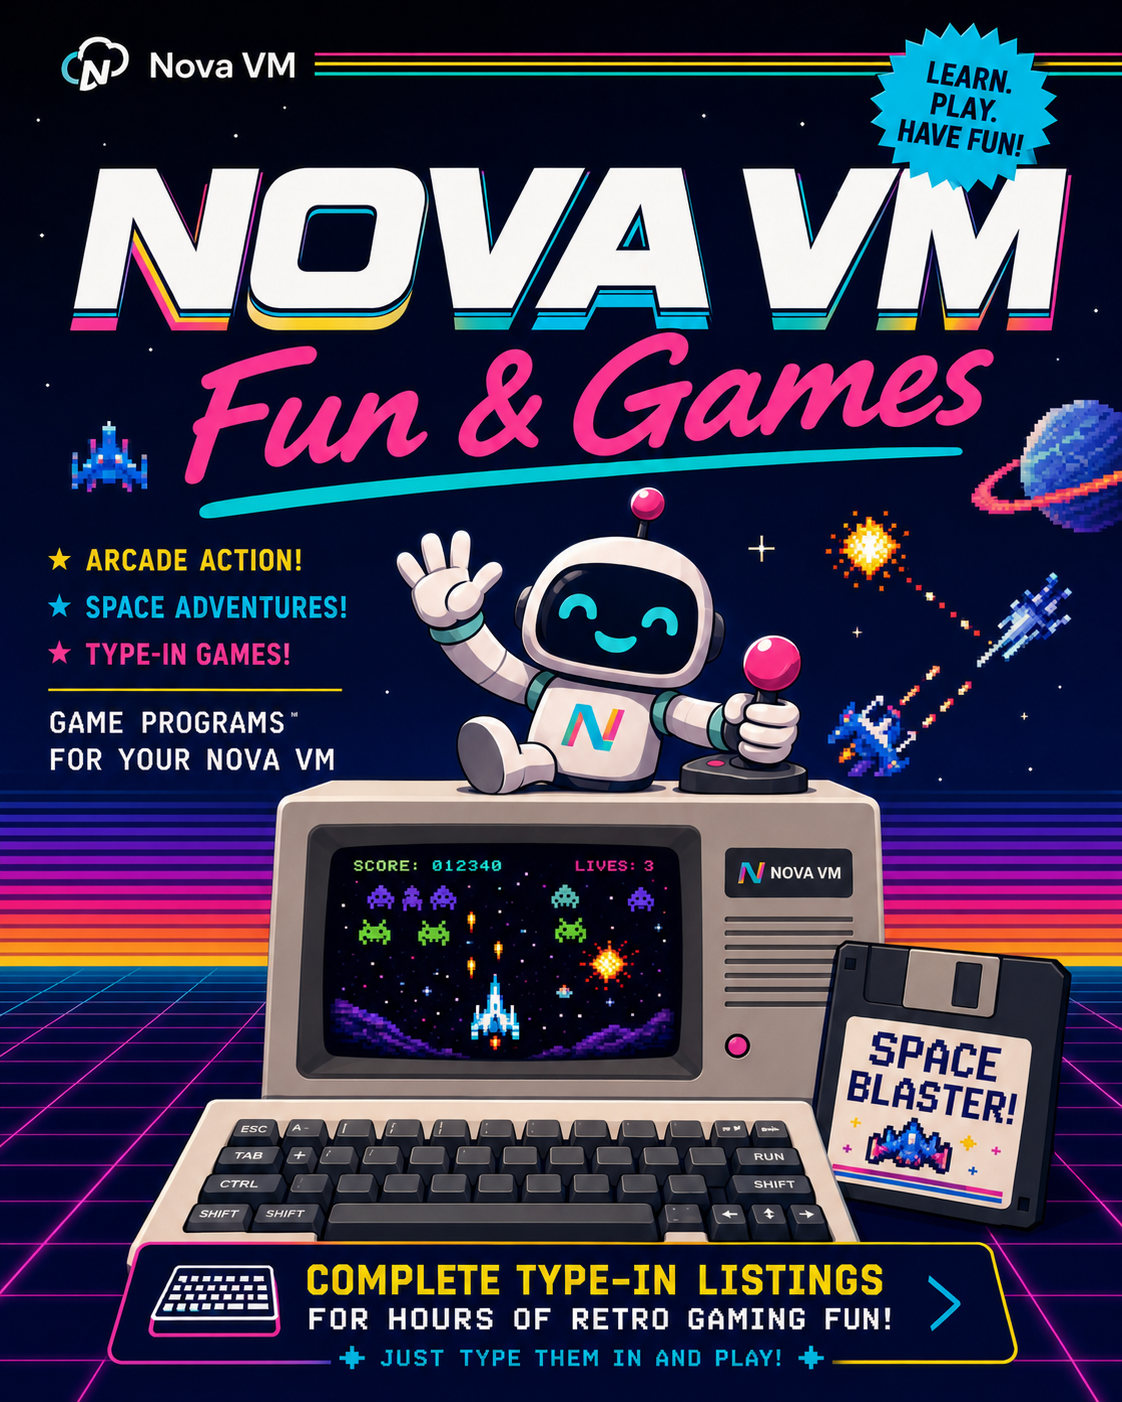
\includegraphics[width=\paperwidth]{assets/front-cover.png}};
\end{tikzpicture}
\null
\end{titlepage}
}{%
\begin{titlepage}
\begin{tikzpicture}[remember picture, overlay]

  \fill[novablue] (current page.south west) rectangle (current page.north east);

  \fill[paper]
    ([xshift=42pt, yshift=42pt]current page.south west)
    rectangle
    ([xshift=-42pt, yshift=-42pt]current page.north east);

  \fill[novared]
    ([xshift=42pt, yshift=-42pt]current page.north west)
    rectangle ++(\paperwidth-84pt,-44pt);
  \fill[novagold]
    ([xshift=42pt, yshift=-86pt]current page.north west)
    rectangle ++(\paperwidth-84pt,-10pt);

  \begin{scope}[shift={([xshift=70pt,yshift=-132pt]current page.north west)}]
    \foreach \x/\y/\c in {
      0/0/novablue,18/0/novacyan,36/0/novagold,54/0/novared,
      0/-18/novacyan,18/-18/novagold,36/-18/novared,54/-18/novagreen,
      0/-36/novagold,18/-36/novared,36/-36/novagreen,54/-36/novablue}
      \fill[\c] (\x pt,\y pt) rectangle ++(13pt,-13pt);
  \end{scope}

  \node[
    anchor=north west,
    xshift=78pt,
    yshift=-176pt,
    text=novablue,
    font=\fontsize{42}{44}\selectfont\bfseries\sffamily,
    align=left
  ] at (current page.north west) {NOVA\\FUN};

  \node[
    anchor=north west,
    xshift=78pt,
    yshift=-270pt,
    text=novared,
    font=\fontsize{42}{44}\selectfont\bfseries\sffamily,
    align=left
  ] at (current page.north west) {\& GAMES};

  \node[
    anchor=north west,
    xshift=82pt,
    yshift=-366pt,
    text=ink,
    font=\fontsize{14}{18}\selectfont\sffamily,
    align=left
  ] at (current page.north west)
    {Type-in programs for NovaBASIC\\
     and the Nova VM};

  \node[
    anchor=north west,
    xshift=82pt,
    yshift=-430pt,
    text=softgray,
    font=\fontsize{10}{14}\selectfont\sffamily,
    align=left
  ] at (current page.north west)
    {Volume 1: Framework, starters, and machine-native game plans};

  \begin{scope}[shift={([xshift=-158pt,yshift=206pt]current page.south east)}]
    \fill[novagreen] (0,0) rectangle (112pt,112pt);
    \fill[paper] (16pt,16pt) rectangle (96pt,96pt);
    \fill[novablue] (32pt,32pt) rectangle (80pt,80pt);
    \fill[novared] (44pt,44pt) rectangle (68pt,68pt);
    \fill[novagold] (52pt,52pt) rectangle (60pt,60pt);
  \end{scope}

  \draw[novablue, line width=2pt]
    ([xshift=62pt,yshift=96pt]current page.south west)
    -- ([xshift=-62pt,yshift=96pt]current page.south east);

  \node[
    anchor=south,
    yshift=60pt,
    text=novablue,
    font=\fontsize{9}{12}\selectfont\sffamily\bfseries
  ] at (current page.south)
    {Graphics | Sprites | Sound | XRAM | File I/O | NovaBASIC};

\end{tikzpicture}
\end{titlepage}
}
